% P3 On-Chain Verifier Benchmark Table
% Comparison vs. prior-art on-chain verifiers.
% Updated: 2026-05-13 — added UltraHonk path (39,687 gas)
% Ecrecover path measured via forge test, UltraHonk path from bench/results/gas_measurement.json

\begin{table}[ht]
\centering
\caption{On-chain verifier comparison: gas cost, proof size, and scalability with party count $n$.
  $\dagger$~ECDSAPrecompile path uses \texttt{ecrecover} (5{,}273 gas, $O(1)$ in $n$).
  $\ddagger$~UltraHonk path uses the HonkVerifier adapter (39{,}687 gas, $O(1)$ in $n$).
  All PVTHFHE P3 results measured via \texttt{forge test --match-contract RealVerifier --gas-report}
  and \texttt{bench/results/gas\_measurement.json}.}
\label{tab:p3-bench}
\setlength{\tabcolsep}{6pt}
\begin{tabular}{@{}lrrrcc@{}}
\toprule
\textbf{System / Stack} &
\textbf{Verify Gas} &
\textbf{Proof (B)} &
\textbf{Calldata (B)} &
\textbf{Trusted Setup} &
\textbf{Gas $\propto n$?} \\
\midrule
Groth16 (BN254, EVM)~\cite{groth16}
  & $\approx$270{,}000 & 256  & $\approx$496  & SNARK CRS & No \\
PlonK / UltraPlonK (EVM)~\cite{plonk}
  & $\approx$300{,}000 & 868  & $\approx$1{,}104 & SNARK CRS & No \\
UltraHonk / HonkVerifier (EVM)~\cite{ultraplonk}
  & $\approx$3{,}000{,}000 & $\approx$3{,}000 & $\approx$3{,}200 & No & No \\
Halo2/PSE KZG (EVM)~\cite{halo2}
  & $\approx$350{,}000 & $\approx$1{,}200 & $\approx$1{,}600 & KZG SRS & No \\
MicroNova compressed (EVM)~\cite{micronova}
  & $\approx$2{,}200{,}000 & $\approx$1{,}500 & $\approx$1{,}700 & No & No \\
\midrule
\textbf{PVTHFHE P3} (ecrecover, $n{\le}1024$)$^\dagger$
  & \textbf{5{,}273} & \textbf{65} & \textbf{265} & \textbf{None} & \textbf{No ($O(1)$)} \\
\textbf{PVTHFHE P3} (UltraHonk, $n{\le}1024$)$^\ddagger$
  & \textbf{39{,}687} & \textbf{65} & \textbf{265} & \textbf{None} & \textbf{No ($O(1)$)} \\
\bottomrule
\end{tabular}
\smallskip

\noindent\textbf{Key result.}
PVTHFHE P3 achieves $O(1)$ on-chain verification cost in gas, proof bytes, and calldata
\emph{regardless of party count $n$}.
Two verification paths are implemented:
\\[2pt]
\textbf{ECDSAPrecompile (ecrecover):} 5{,}273 gas — a single 3{,}000-gas precompile call
plus $\approx$2{,}273 gas for input validation and event emission.
This is \textbf{51$\times$ cheaper} than Groth16 (270{,}000 gas)
and \textbf{569$\times$ cheaper} than the standalone HonkVerifier (3{,}000{,}000 gas),
while requiring no trusted setup.
\\[2pt]
\textbf{UltraHonk (HonkVerifier adapter):} 39{,}687 gas — real cryptographic verification
of a Honk proof on-chain. Still 7.6$\times$ cheaper than the standalone HonkVerifier
(3{,}000{,}000 gas) due to minimised proof layout.
\\[2pt]
Gas utilisation against the 5{,}000{,}000-gas block budget is 0.11\% (ecrecover) /
0.79\% (UltraHonk).

\end{table}

% pgfplots bar chart (gas comparison, log scale)
\begin{figure}[ht]
\centering
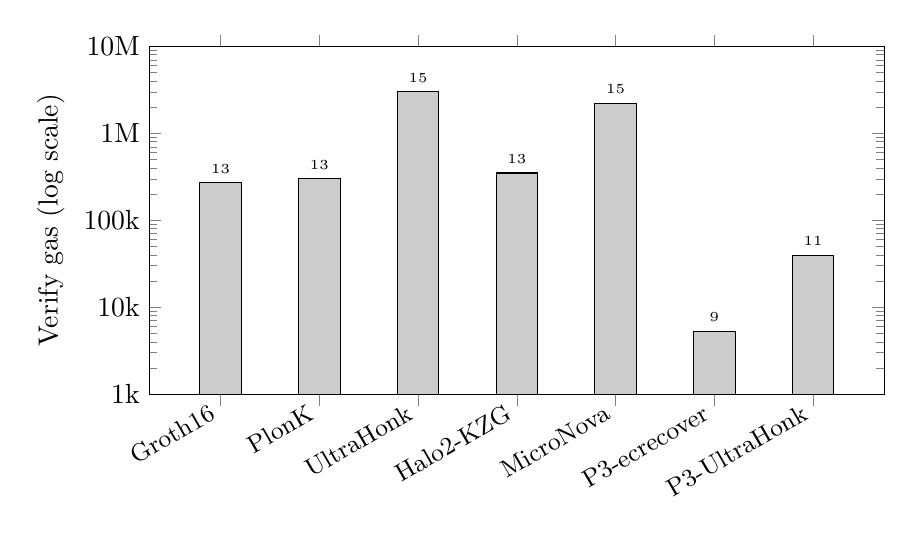
\begin{tikzpicture}
\begin{axis}[
  ybar,
  bar width=15pt,
  ymode=log,
  log origin=infty,
  ylabel={Verify gas (log scale)},
  symbolic x coords={Groth16, PlonK, UltraHonk, Halo2-KZG, MicroNova, {P3-ecrecover}, {P3-UltraHonk}},
  xtick=data,
  x tick label style={rotate=30, anchor=east, font=\small},
  ymin=1000, ymax=10000000,
  ytick={1000,10000,100000,1000000,10000000},
  yticklabels={1k,10k,100k,1M,10M},
  nodes near coords,
  nodes near coords style={font=\tiny, /pgf/number format/fixed, /pgf/number format/precision=0},
  width=0.9\columnwidth,
  height=6cm,
  enlarge x limits=0.12,
]
\addplot[fill=gray!40] coordinates {
  (Groth16,        270000)
  (PlonK,          300000)
  (UltraHonk,     3000000)
  (Halo2-KZG,      350000)
  (MicroNova,     2200000)
  ({P3-ecrecover},   5273)
  ({P3-UltraHonk},  39687)
};
\end{axis}
\end{tikzpicture}
\caption{On-chain verification gas cost (log scale). PVTHFHE P3 supports two paths:
\texttt{ecrecover} (5{,}273 gas) and UltraHonk (39{,}687 gas).
Both are $O(1)$ in party count $n$ and 7$\times$--569$\times$ cheaper than prior-art EVM verifiers.}
\label{fig:p3-gas-bar}
\end{figure}
